\begin{figure}[htb!] % Posición de la figura en la página
\centering % Centrar la figura
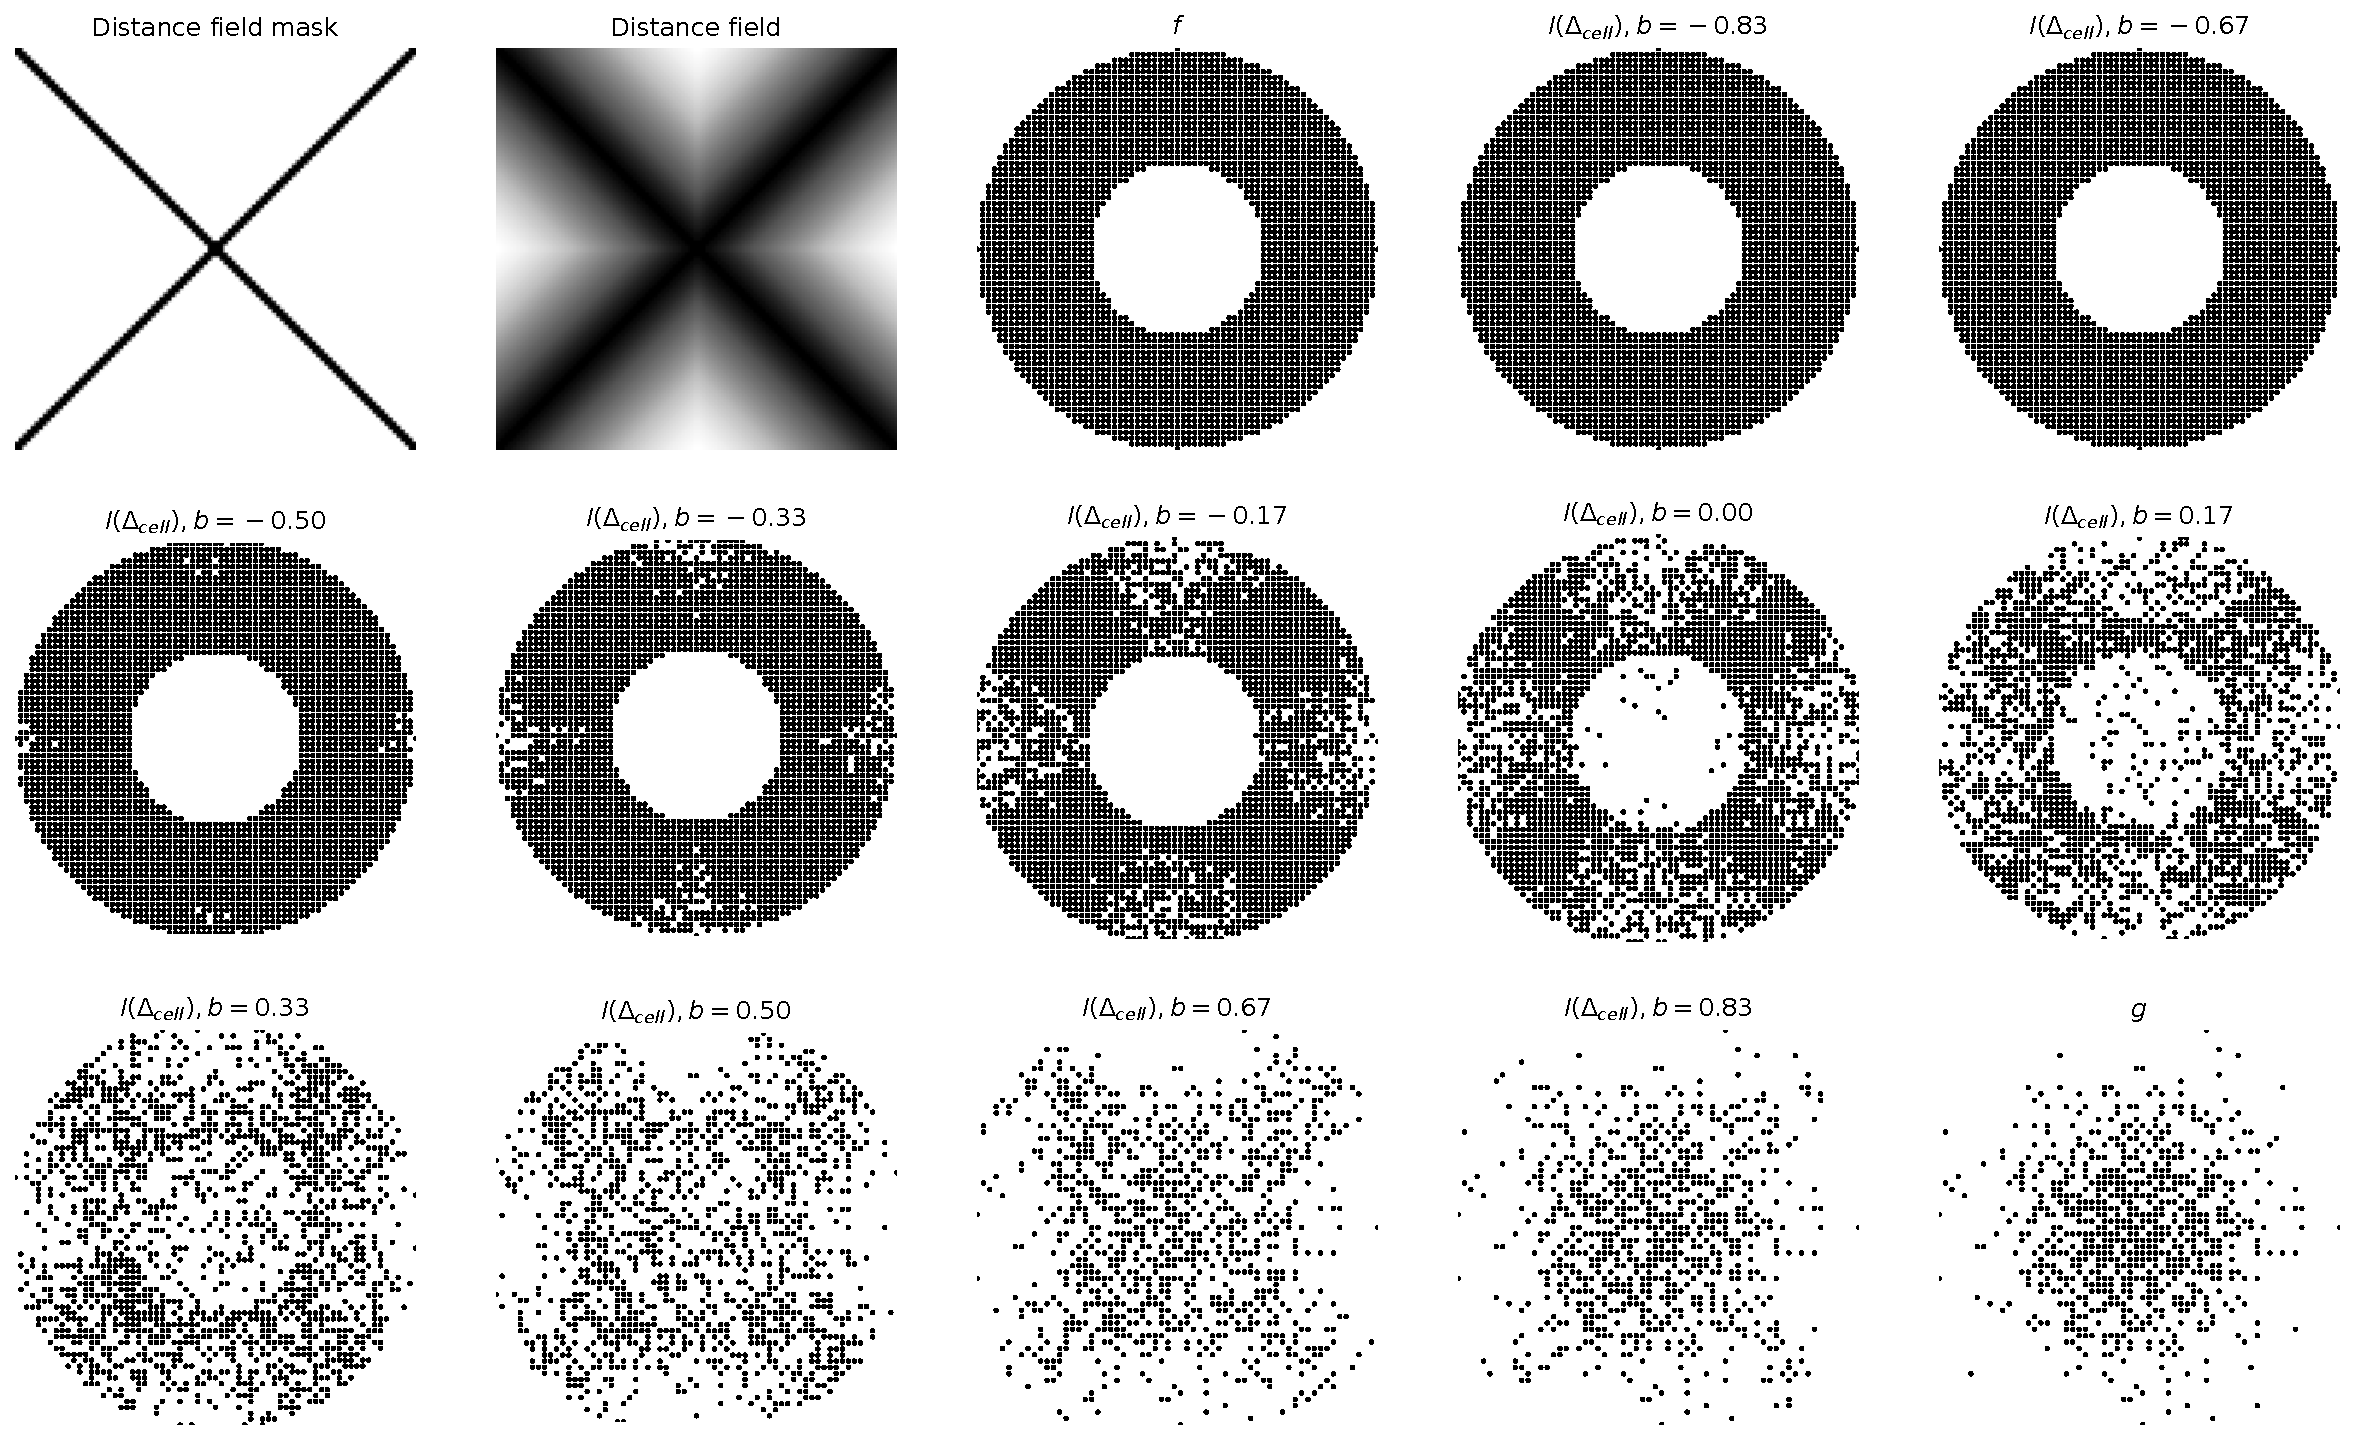
\includegraphics[width=\textwidth]{test-distribuciones}
\caption[Lista de distribuciones]{Lista de distribuciones: Aquí iría una descripción de la figura para cada fila o columna, explicando los parámetros. Fíjate como el pie está recortado en el índice para que no sea extremadamente largo. Si hay una fuente, la podemos colocar aquí: \url{https://drive.google.com/file/d/14YN87TAF6OQq6JIuZiUz3YHn-6Pz8KHm/view?usp=sharing}}
\label{fig:grafica} % Etiqueta de referencia para la figura
\end{figure}
